\documentclass[12pt]{beamer} %slightly bigger font
\usetheme{default} % other themes are available; 'default' is fine, & simple

\setbeamertemplate{navigation symbols}{} %gets rid of navigation symbols
\setbeamertemplate{footline}{} %gets rid of bottom navigation bars
%\setbeamertemplate{footline}[page number]{} %use this, if you want page numbers

\setbeamertemplate{itemize items}[circle] %I like round bullet points
\setlength\parskip{10pt} % I like white space between paragraphs

% I will abuse the section/subsection/frame labeling system
% - I just use frame labels, not sections and subsections
% Here is a `helper' functions to save typing, later

\setbeamertemplate{frametitle continuation}[from second][ ]
\newcommand{\mystart}[1]{ \section{#1}\begin{frame}[allowframebreaks] \frametitle{#1} } 

% information for the title slide
\title{Some \texttt{beamer} examples } % title infomation
\author{Ken Rice}
\institute{STAT/BIOST 572}
\date{\today}

% This concludes the preamble. Now to start the 'proper' document;
\begin{document}

\begin{frame} %start a new slide
  \titlepage %puts the title information on a pretty title page
\end{frame} %end the slide; don't forget this

%here's the first proper slide; (the 'mystart' command include 'begin{frame}')
\mystart{Outline}
  \begin{itemize} % i.e. a bulleted list
  \item Your talks, and why they're useful
  \item Planning your talk
  \item Making slides, and graphs
  \item Giving your talk
  \end{itemize}
See also resources, on the class site

Note: I'll give \textit{some} essentials, mostly just advice. Aim to acquire out a presentation style that works for you

\end{frame} %don't forget this! (I always do)

%now for the second proper slide
\mystart{Your talks}
In 572, you'll give three talks;
  \begin{enumerate} % a numbered list
  \item \textbf{Brief overview:} (15 mins) What the paper does, the problem it addresses, and how the papers fits into the literature
  \item \textbf{Update:} (15 mins) What you've figured out, what you still need to do
  \item \textbf{Final:} (20 mins) Full summary of the paper, and your critique
  \end{enumerate} 
Giving a talk \textbf{forces} you to `make sense' of the material; in your own mind, and the audience's

For short talks you must figure out and give the `essence' of the material -- detailed knowledge is required, but is not the focus of the presentation

% the third slide just continues the previous one
\pagebreak %starts a new slide, but with the same frametitle

Greg Dyke is the bald guy on the `BS' slide
\begin{itemize}
\item He was Director General of the BBC, so knows a bit about effective communication
\item He got annoyed at TV producers BSing
\item His `Cut the Crap' cards were meant to operate like yellow cards (i.e. warnings) in soccer; pull one from your pocket, wave it, and shame the recipient into better behavior
\end{itemize}

\end{frame}
\mystart{A slide with a picture in it}

A \textit{really horrible} pie chart

\begin{center}
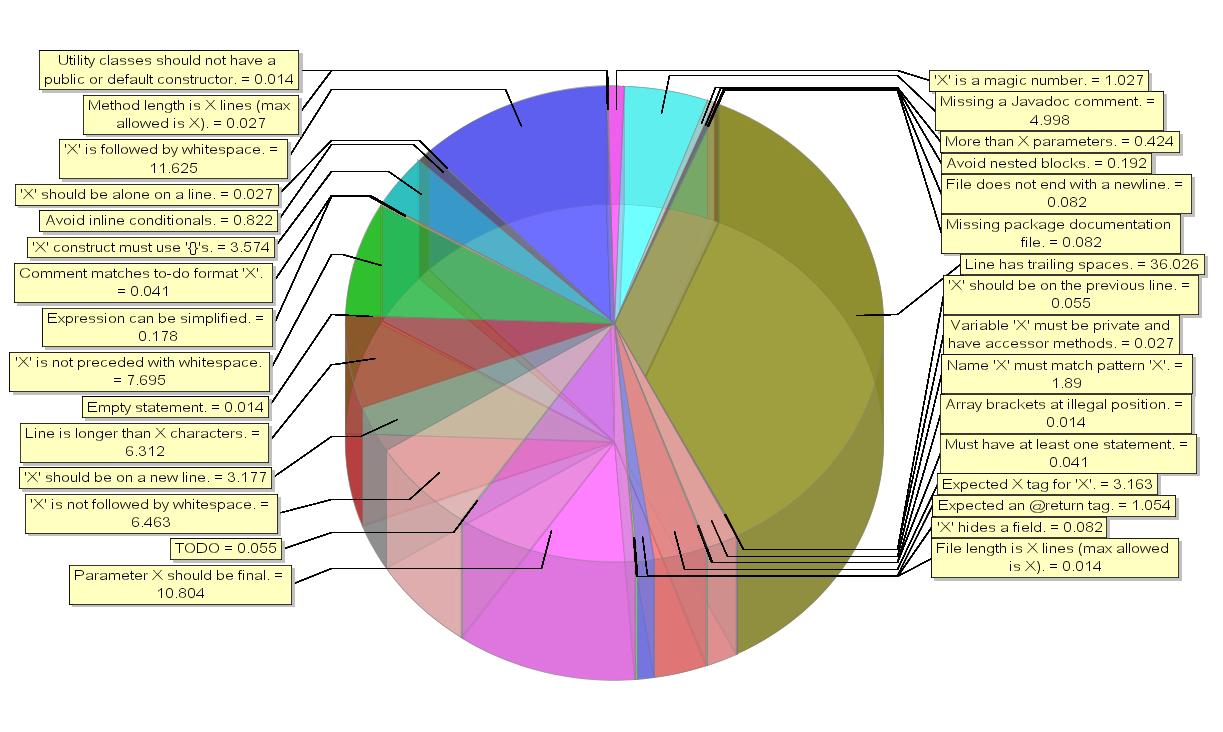
\includegraphics[height=0.65\textheight]{horridpie1.jpg} 
\end{center}

\end{frame}
\mystart{A slide with several pictures}

\raisebox{-0.3in}{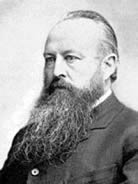
\includegraphics[height=0.8in]{acton.jpg}}~~\begin{minipage}{3.8in}
\textit{Power corrupts. \\ Absolute power corrupts absolutely}
\begin{flushright}
Baron John Acton (1834--1902) Historian and Moralist
\end{flushright}\end{minipage}

\raisebox{-0.3in}{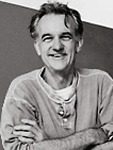
\includegraphics[height=0.8in]{tufte.jpg}}~~\begin{minipage}{3.8in}
\textit{Power corrupts. \\ PowerPoint corrupts absolutely}
\begin{flushright}
Edward Tufte (1942-- ) Graphics Guru and Statistician
\end{flushright}\end{minipage}

\begin{itemize}
  \item I used \texttt{$\backslash$minipage}, \texttt{$\backslash$includegraphics}  and \texttt{$\backslash$raisebox} to make this
  \item \texttt{$\backslash$begin\{tabular\}...$\backslash$end\{tabular\}} can also work
  \item Like \texttt{R}, there are loads of ways to do these little jobs in \LaTeX. Use mine if you like, but anything that works is worthwhile
\end{itemize}

\end{frame}

\begin{frame}
\begin{itemize}
\item<1-> from first layer on
\item<2-> from second layer on
\item<4>  only in the 4. layer
\item<3,5-> in the 3., 5. and all further layers
\end{itemize}
\end{frame}

\end{document} % don't forget this

